%%%%%%%%%%%%%%%%%%%%%%%%%%%%%%%%%%%%%%%%%%%%%%%%%%%%%%%%%%%%%%%%%%%%%%%%%%% 
% 
% Generic template for TFC/TFM/TFG/Tesis
% 
% By:
% + Javier Macías-Guarasa. 
% Departamento de Electrónica
% Universidad de Alcalá
% + Roberto Barra-Chicote. 
% Departamento de Ingeniería Electrónica
% Universidad Politécnica de Madrid   
% 
% Based on original sources by Roberto Barra, Manuel Ocaña, Jesús Nuevo,
% Pedro Revenga, Fernando Herránz and Noelia Hernández. Thanks a lot to
% all of them, and to the many anonymous contributors found (thanks to
% google) that provided help in setting all this up.
% 
% See also the additionalContributors.txt file to check the name of
% additional contributors to this work.
% 
% If you think you can add pieces of relevant/useful examples,
% improvements, please contact us at (macias@depeca.uah.es)
% 
% You can freely use this template and please contribute with
% comments or suggestions!!!
% 
%%%%%%%%%%%%%%%%%%%%%%%%%%%%%%%%%%%%%%%%%%%%%%%%%%%%%%%%%%%%%%%%%%%%%%%%%%% 

\chapter{Related Works}
\label{cha:related_works}

begin{FraseCelebre}
\begin{Frase}
	Llegaré a ser el mejor, El mejor que habrá jamás \\
	Mi causa es ser su entrenador, Tras poderlos capturar.  
	
	Viajaré a cualquier lugar, Llegaré a cualquier rincón \\  
	Y al fin podré desentrañar, El poder de su interior.  
	
	¡Pokémon! Hazte con todos (solos tú y yo), \\
	Es mi destino, mi misión \\
	¡Pokémon! Tú eres mi amigo fiel, \\
	Nos debemos defender.
\end{Frase}
\begin{Fuente}
	Opening 1 de Pokémon: "Gotta catch 'em all!" \\
	Autor original: Jason Paige
\end{Fuente}
\end{FraseCelebre}

\begin{comment}
	TODO:
	1. Hacer intro general
	2. CBP vs PMP (https://ieeexplore.ieee.org/stamp/stamp.jsp?tp=&arnumber=9981524)
	3. Problem Formulation
	4. Contextual
	5. Classification
	5.1. Physics  (1)
	5.2. Machine Learning (1)
	5.2. Deep Learning (4)
	5.3. Reinforcement Learning (1)
	5.4. Comparison
	6. Some particular methods of interest of DL (CRAT-PRED, LaneGCN, GANet) -> Destacar puntos débiles
\end{comment}

One of the crucial tasks that \acp{ADS} must face during navigation, specially in arbitrarily complex urban scenarios, is to predict the behaviour of dynamic obstacles \cite{chang2019argoverse, salzmann2020trajectron++}. In a similar way to humans that pay more attention to nearby obstacles and upcoming turns than considering the obstacles far away, the perception layer of an \ac{ADS} must focus more on the salient regions of the scene, particularly on the more relevant dynamic agents to predict their future behaviour before conducting a maneuver, such as lane changing or accelerating. \\ 

CONTINUAR








Most traditional predictions methods \cite{huang2022survey}, which usually only consider physics-related factors (like the velocity and acceleration of the target vehicle that is going to be predicted) and road-related factors (prediction as close as possible to the road centerline), are only suitable for \textbf{short-time} prediction tasks \cite{huang2022survey} and simple traffic scenarios, such as constant velocity (CV) in a highway or a curve (Constant Turn Rate Velocity, CTRV) where a single path is allowed, i.e. multiple choices computation are not required. Recently, MP methods based on DL have become increasingly popular since they are able not only to take into account these above-mentioned factors but also consider interaction-related factors (like agent-agent \cite{gupta2018social}, agent-map \cite{casas2018intentnet} and map-map \cite{liang2020learning}) in such a way the algorithm can adapt to more complex traffic scenarios (intersections, sudden breaks and accelerations, etc.). It must be consider that multimodal, specially in the field of vehicle motion prediction, does not refer necessarily to different directions (e.g. turn to the left, turn to the right, continue forward in an intersection), but it may refer to different predictions in the same direction that model a sudden positive or negative acceleration, so as to imitate a realistic human behaviour in complex situations. As expected, neither classical nor Machine Learning (ML) methods can model these situations \cite{huang2022survey}.

\begin{table*}[t]
	\begin{center}
		\caption{Main state-of-the-art methods for Motion Prediction. Main categories are Encoder (splitted into motion history, social info (agent interactions) and map info (physical information)), Decoder, Output representation and Distribution over future trajectories.}
		%\begin{tabular}{| c | cccccc |}
		%\begin{tabular}{| c | cccccc |}
		\begin{tabular}{r |ccc|c|c|c}
			
			\toprule
			\textbf{Method}	&	& \textbf{Encoder}	&	& \textbf{Decoder}	& \textbf{Output}  & \textbf{Trajectory Distribution}	\\
			& Motion history	& Social info	& Map info	&	&	&	\\
			\midrule
			\midrule
			SocialLSTM~\cite{alahi2016social}	& LSTM	& spatial pooling	& --	& LSTM	& states	& samples	\\
			SocialGan~\cite{gupta2018social}	& LSTM	& maxpool	& --	& LSTM	& states	& samples	\\
			Jean~\cite{mercat2020multiattentmotion}	& LSTM	& attention	& --	& LSTM	& states	& GMM	\\
			TNT~\cite{zhao2020tnt}	& polyline	& maxpool, attention	& polyline	& MLP	& states	& weighted set	\\
			LaneGCN~\cite{liang2020learninggraph}	& 1D-conv	& GNN	& GNN	& MLP	& states	& weighted set	\\
			WIMP~\cite{khandelwal2020if}	& LSTM	& GNN+attention	& polyline	& LSTM	& states	& GMM	\\
			VectorNet~\cite{gao2020vectornet}	& polyline	& maxpool, attention	& polyline	& MLP	& states	& unimodal	\\
			SceneTransformer~\cite{ngiam2021scene}	& attention	& attention	& polyline	& attention	& states	& weighted set	\\
			HOME~\cite{gilles2021home}	& raster	& attention	& raster	& conv	& states	& heatmap	\\
			GOHOME~\cite{gilles2021gohome}	& 1D-conv+GRU	& GNN	& GNN	& MLP	& states	& heatmap	\\
			MP3~\cite{casas2021mp3}	& raster	& conv	& raster	& conv	& cost function	& weighted samples	\\
			%CoverNet~\cite{phan2019covernet}	& raster	& conv	& raster	& lookup	& states	& GMM w/ dynamic anchors	\\
			%DESIRE~\cite{lee2017desire}	& GRU	& spatial pooling	& raster	& GRU	& states	& samples	\\
			ExploringGAN~\cite{gomez2022exploring}	& LSTM	& attention	& polyline	& LSTM	& states	& unimodal	\\
			% MFP~\cite{tang2019multiple}	& GRU	& RNNs+attention	& raster	& GRU	& states	& samples	\\
			%MANTRA~\cite{marchetti2020mantra}	& GRU	& --	& raster	& GRU	& states	& samples	\\
			%PRANK~\cite{biktairov2020prank}	& raster	& conv	& raster	& lookup	& states	& weighted set	\\
			%IntentNet~\cite{casas2018intentnet}	& raster	& conv	& raster	& conv	& states	& unimodal	\\
			Multimodal~\cite{cui2019multimodal}	& raster	& conv	& raster	& conv	& states	& weighted set	\\
			MultiPath~\cite{chai2019multipath}	& raster	& conv	& raster	& MLP	& states	& GMM w/ static anchors	\\
			MultiPath++~\cite{varadarajan2021multipath++}	& LSTM	& RNNs+maxpool	& polyline	& MLP	& control poly	& GMM	\\
			%PLOP~\cite{buhet2021plop}	& LSTM	& conv	& raster	& MLP	& state poly	& GMM	\\
			Trajectron++\cite{salzmann2020trajectron++}	& LSTM	& RNNs+attention	& raster	& GRU	& controls	& GMM	\\
			CRAT-PRED\cite{schmidt2022crat}	& LSTM	& GNN+attention	& --	& MLP	& states	& weighted set	\\
			%R2P2~\cite{rhinehart2018r2p2}	& GRU	& --	& polyline	& GRU	& motion	& samples	\\
			%DKM~\cite{cui2020deep}	& raster	& conv	& raster	& conv	& controls	& weighted set	\\
			\midrule					
			\textbf{Ours - Social baseline}	& LSTM	& GNN+attention	& --	& LSTM	& states	& weighted samples	\\
			\textbf{Ours - Map baseline}	& LSTM	& GNN+attention	& polyline 	& LSTM	& states	& weighted samples	\\
			\bottomrule
		\end{tabular}
		\label{table:related_work}
	\end{center}
\end{table*} 

In order to classify DL based MP methods, we distinguish several important features: Motion history, Social information (agent interactions), Map information (road encoding), how the model returns the output trajectory and its corresponding distribution. Table \ref{table:related_work} summarizes several SOTA methods, inspired in the survey proposed by \cite{varadarajan2021multipath++}.

\begin{itemize}
	
	\item \textbf{Motion history}: Most methods encode the sequence of past observed states using 1D-convolution \cite{liang2020learninggraph} \cite{mercat2020multiattentmotion}, able to model spatial information, or via a recurrent net \cite{gomez2022exploring} \cite{alahi2016social} (LSTM, GRU), which are more useful to handle temporal information. Other methods that use a raster version of the whole scenario represent the agent states rendered as a stack of binary mask images depicting agent oriented bounding boxes \cite{gilles2021home}. On the other hand, other approaches encode the past history of the agents in a similar way to the road components of the scene given a set of vectors or polylines \cite{zhao2020tnt, gao2020vectornet} that can model the high-order interactions among all components, or even employing attention to combine features across road elements and agent interactions \cite{ngiam2021scene}.
	
	\item \textbf{Social information}: In complex scenarios, motion history encoding of a particular target agent is not sufficient to represent the latent space of the traffic situation, but the algorithm must deal with a dynamic set of neighbouring agents around the target agent. Common techniques are aggregating neighbour motion history with a permutation-invariant set operator: soft attention \cite{ngiam2021scene, gomez2022exploring}, a combination of soft attention and RNN \cite{varadarajan2021multipath++} / GNN \cite{schmidt2022crat} or social pooling \cite{alahi2016social, gupta2018sgan}. Raster based approaches rely on 2D convolutions \cite{chai2019multipath} \cite{casas2021mp3} over the spatial grid to implicitly capture agent interactions in such a way long-term interactions are dependent on the neural network receptive fields.
	
	%quito la cita suelta \cite{murciego2018topological} para evitar self-citations en review y ahorrar 4 lineas. En el CR la puedes añadir.
	
	\item \textbf{Map information}: High-fidelity maps~\cite{can2022maps} have been widely adopted to provide offline information (also known as physical context) to complement the online information provided by the sensor suite of the vehicle and its corresponding algorithms. Recent learning-based approaches \cite{mahjourian2022occupancy, casas2018intentnet, ivanovic2021heterogeneous}, which present the benefit of having probabilistic interpretations of different behaviour hypotheses, require to build a representation to encode the trajectory and map information. Map information is probably the feature with the clearest dichotomy: raster vs vector treatment. The raster approach encodes the world around the particular target agent as a stack of images (generally from a top-down orthographic view, also known as Bird's Eye View). This world encoding may include from agent state history, agent interactions and usually the road configuration, integrated all this different-sources information as a multi-channel image \cite{gilles2021home}, in such a way the user can use an off-the-shelf Convolutional Neural Network (CNN) based pipeline in order to leverage this powerful information. Nevertheless, this representation has several downsides: constrained field of view, difficulty in modeling long-range interactions and even difficulty in representing continuous physical states due to the inherent world to image (pixel) discretization. On the other hand, the polyline approach may describe curves, such as lanes, boundaries, intersections and crosswalks, as piecewise linear segments, which usually represents a more compact and efficient representation than using CNNs due to the sparse nature of road networks. Some state-of-the-art algorithms not only describe the world around a particular agent as a set-of-polylines \cite{khandelwal2020if} \cite{zhao2020tnt} in an agent-centric coordinate system, but they also leverage the road network connectivity structure \cite{liang2020learninggraph} \cite{zeng2021lanercnn} treating road lanes as a set of nodes (waypoints) and edges (connections between waypoints) in a graph neural network so as to include the topological and semantic information of the map.
	
	% Additional bio: deo2018cstlstmpool, rhinehart2019precog
	
	\item \textbf{Decoder}: Pioneering works of DL based MP usually adopt the autoencoder architecture, where the decoder is often represented by a recurrent network (GRU, LSTM, etc., specially designed to handle temporal information) to generate future trajectories in an autoregressive way, or by CNNs \cite{gilles2021home} \cite{gilles2021gohome} / MLP \cite{liang2020learninggraph} \cite{schmidt2022crat} using the non-autoregressive strategy. The method may use an autoregressive strategy where the pipeline generates tokens (in this case, positions or relative displacements) in a sequential manner, in such a way the new output is dependent on the previously generated output, whilst MLP \cite{schmidt2022crat}, CNN \cite{gilles2021home} or transformer \cite{ngiam2021scene} based strategies usually follow a non-autoregressive strategy, where from a latent space the whole future trajectory is predicted.
	
	\item \textbf{Output}: The most popular model output representation is a sequence of states (absolute positions) or state differences (relative displacements for any dimension considered). The spacetime trajectory may be intrinsically represented as a continous polynomial representation or a sequence of sample points. Other works \cite{gilles2021home} \cite{gilles2021gohome} first predict a heatmap and then decode the corresponding output trajectories after sampling points from the heatmap, whilst \cite{casas2021mp3} \cite{zeng2019end} learn a cost function evaluator of trajectories that are enumerated heuristically instead of being generated by a learned model. 
	
	\item \textbf{Trajectory Distribution}: The choice of output trajectory distributions has several approaches on downstream applications. Regardless the agent to be predicted is described as a (non-)holonomic \cite{triggs1993motion} platform, an intrinsic property of the motion prediction problem is that the agent must follow one of a diverse set of possible future trajectories. A popular choice to represent a multimodal prediction are Gaussian Mixture Models (GMMs) due to their compact parameterized form, where mode collapse (associated frequently to GMMs) is addressed through the use of trajectory anchors \cite{chai2019multipath} or training  tricks \cite{cui2019multimodal}. Other approaches model a discrete distribution via a collection of trajectory samples extracted from a latent space and decoded by the model \cite{rhinehart2018r2p2} or over a set of trajectories (fixed or a priori learned) \cite{liang2020learninggraph}.
	
	% Additional bio: \cite{biktairov2020prank}
	
\end{itemize}

After classifying main SOTA methods, we conclude this section presenting the main characteristics of our baseline approaches. We make use of LSTM to encode the past motion history, GNN in combination with soft-attention the compute social interactions, a set-of-polylines to represent the most important map information and LSTM to decode the trajectories from the latent space. The output multimodal prediction is represented by a set of states with their corresponding confidences indicating the most plausible modes.
% Social LSTM \cite{alahi2016social} applies an LSTM autoencoder (adopting the NLL loss to model the error for each future step) whilst its generative continuation, Social GAN \cite{gupta2018social} uses an adversarial \cite{goodfellow2014gan} frame with social attention encoding the input trajectories with LSTM and then decoding different multiple modalities with the inherent noise associated to generative models, adopting per-step MSE loss. DESIRE \cite{lee2017desire} applies a conditional variational autoencoder in order to sample a diverse set of plausible modalities, making use of a GRU to generate the final predictions. 

% Moreover, SoPhie \cite{sadeghian2019sophie} represents one of the first DL based MP models that leverages two sources of information: the path states (position, velocity, heading, etc.) of all the agents in the scene and the physical context information, using Bird's Eye View (BEV) images as inputs and CNN as feature extractor. After fusing both physical and social attention, this model can successfully predict multiple acceptable trajectories that respect both social constraints (not collide with other agents) and physical constraints (most predictions are in the plausible area). Authors show that by modeling jointly the information about the physical environment and interactions between all agents, the model is able to learn better than when both sources of information are used independently

% In that sense, high-fidelity maps~\cite{can2022maps} have been widely adopted to provide offline information (also known as physical context) to complement the online information provided by the sensor suite of the vehicle and its corresponding algorithms. Recent learning-based approaches \cite{mahjourian2022occupancy, xiao2022multimodalend2end, casas2018intentnet, deo2018cstlstmpool, rhinehart2019precog, ivanovic2021heterogeneous}, which present the benefit of having probabilistic interpretations of different behaviour hypotheses, require to build a representation to encode the trajectory and map information. Hong et al.~\cite{hong2019rules} assumes that detections around the vehicle are provided and focuses on behaviour prediction by encoding entity interactions with ConvNets. \textbf{Intentnet}~\cite{casas2018intentnet} proposes to jointly detect traffic participants (mostly focused on vehicles) and predict their trajectories using raw LiDAR pointcloud and HD map information. %PRECOG~\cite{rhinehart2019precog} aims to capture the future stochasticity by flow-based generative models. 
%
% \textbf{MultiPath} by Chai et al.~\cite{chai2019multipath} uses ConvNets as encoder and adopts pre-defined trajectory anchors to regress multiple possible future trajectories.

% \textbf{HOME} by Gilles et al.~\cite{gilles2021home} presented a novel representation for multimodal trajectory prediction, where the model takes as input the context (map) and history of past trajectories, and generates an unconstrained 2D heatmap representation of the agent’s possible future trajectories, which represents the probability distribution of the agent’s future location. The method builds on simple architecture with classic convolution networks coupled with attention mechanism for agent interactions. Fig.~\ref{fig:prev_models} shows the SoPhie and HOME architectures. Both methods have two-streams, one for each input (trajectories and map), and use CNNs to process the map or physical context.

% In Section~\ref{sec:ours} we explain our solution to this trade-off problem.

\

\section{Introduction}
\label{sec:2_introduction}

\begin{figure}[h]
	\centering
	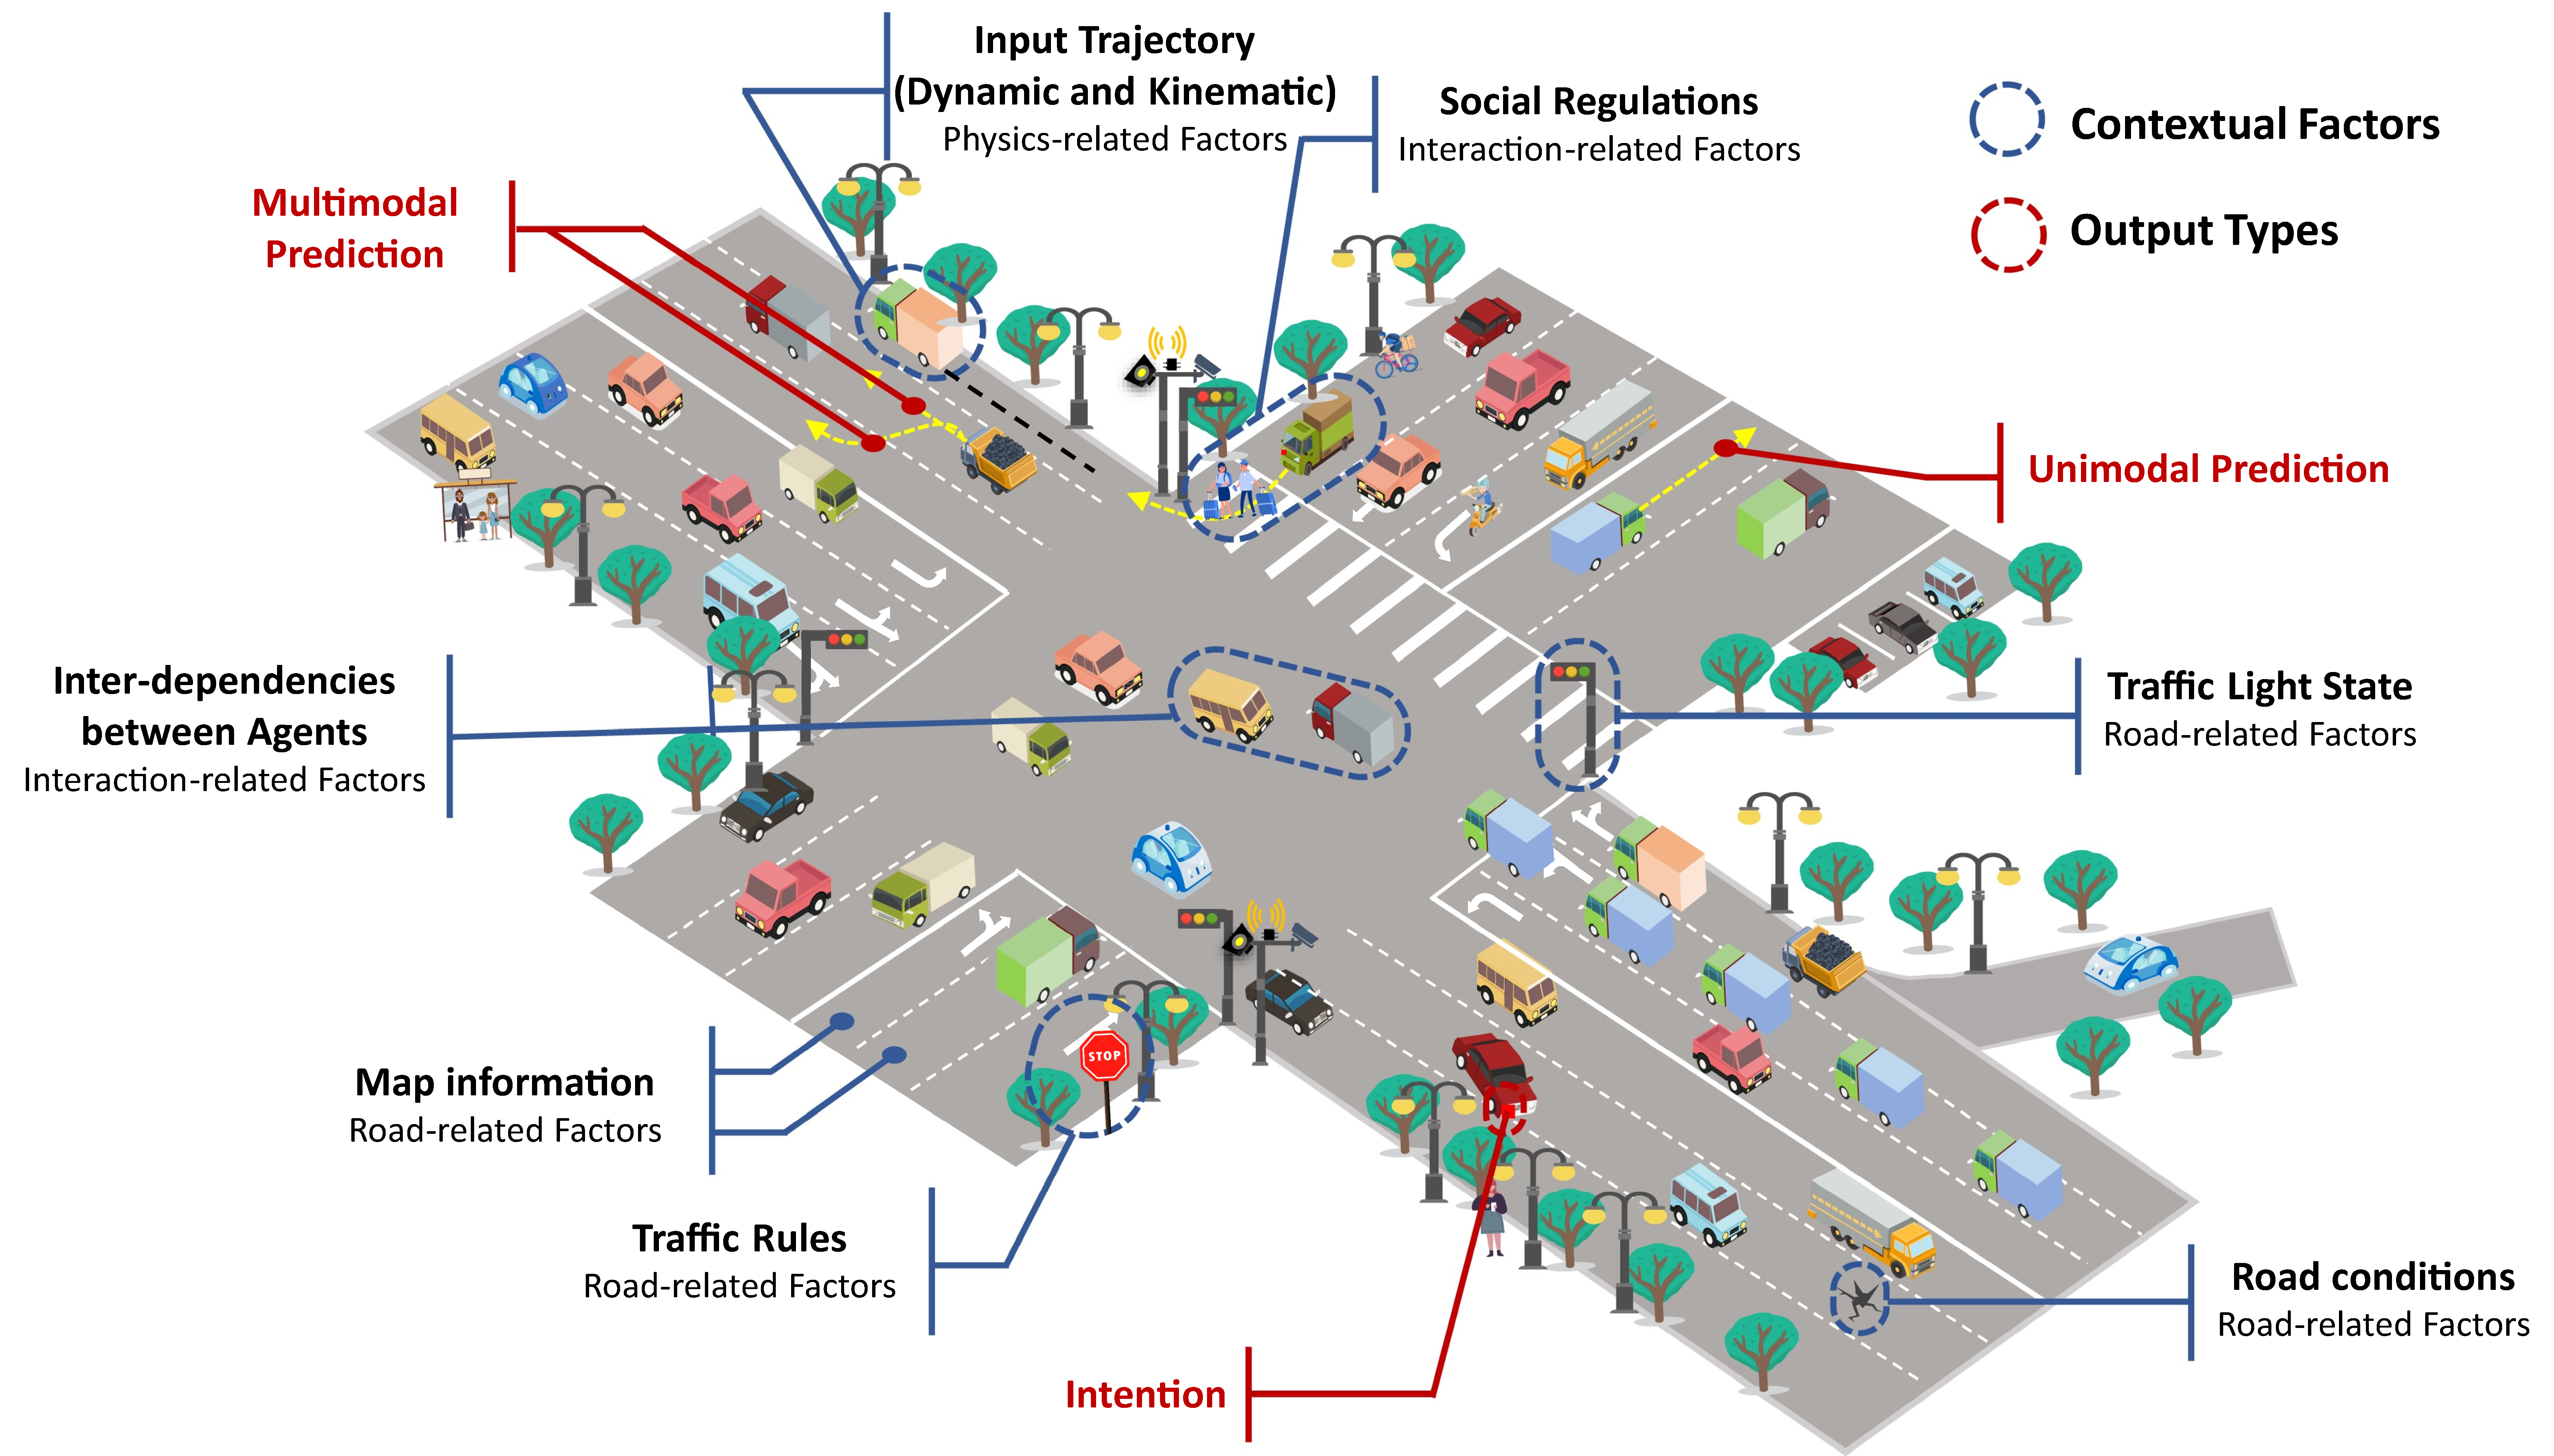
\includegraphics[width=\linewidth]{2_inputs_outputs_mp.pdf}
	\caption{Contextual factors and output types in Vehicle Motion Prediction}
	%Source: \textit{A survey on trajectory-prediction methods for autonomous driving} \cite{huang2022survey}
	\label{fig:2_input_output_map}
\end{figure}



\section{Problem Formulation of Motion Prediction}
\label{sec:2_problem_formulation_mp}

Given a sequence of past trajectories $a_{P}=[a_{-T^{'}+1},a_{-T^{'}+2},...,a_{0}]$ for an agent, we aim to predict its future steps $a_{F}=[a_{1},a_{2},...,a_{T}]$ up to a fixed time step $T$. Running in a specific traffic scenario, each actor will interact with static HD maps $m$ and the other dynamic actors, meeting the corresponding traffic and social rules. Therefore, the probabilistic distribution that we want to capture is $p(a_F|m, a_P, a^O_P)$, where $a^O_P$ denotes the other actors' observed states. One important thing to note is that this thesis is focused on non-conditional motion prediction, different to Conditional Behaviour Prediction (CBP). Most existing works focus on a passive prediction scheme, where the future states of a particular agent are predicted given its past information, other surrounding agents information and interactions as well as the physical context. However, when using such a \ac{MP} model, downstream planning modules, specially the behaviour planning (also referred as decision-making, as stated in Section \ref{sec:1_ad_architecture}), determine the ego-vehicle (our vehicle) action according to the predicted trajectories in a passive manner, that is, without modifying the output of the prediction model. Nevertheless, to ensure safety under various predicted trajectories of the surrounding agents, our vehicle must overly conservative with inefficient maneuvers, especially un highly interactive scenarios, because passive \ac{MP} models ignore the fact that the future actions of an agent can influence the future actions of other agents, what is the most realistic situation. To this end, researchers started to investigate a more coherent interactive prediction and planning framework which relies on predicting the surrounding agents future trajectories conditioned on the ego-vehicle future actions \cite{tang2019multiple} \cite{rhinehart2019precog} \cite{khandelwal2020if}. Under such frameworks, the \acs{ADS} can reason 

surrounding agents’ future trajectories conditioned on the
ego agent’s future actions [3], [4], [5], [6], [7], [8], [9], [10].
Under such frameworks, the autonomous agents can reason
over potential actions while considering their influence on
surrounding agents. It can then induce more efficient and
less conservative maneuvers in interactive scenes. Some of
these prior works merely demonstrated that their models are
able to support conditional prediction from the perspective
of architecture [4], [6]. Another line of works focused on

More interestingly, some existing works formulated an
alternative prediction task to evaluate the prediction module
in a self-contained way [8], [7], [10]. We follow [10] to
refer to this task as conditional behavior prediction (CBP). In
the CBP task, the future trajectories of the target agents are
predicted conditioned on the ground-truth future trajectory
of an assigned ego agent. Standard prediction metrics are
adopted to quantify the performance. It allows us to leverage
large-scale naturalistic traffic datasets to develop and validate
a conditional prediction model before closed-loop testings. In
those works, a model that can achieve the smallest prediction
error after granted the additional future information of the
ego agent is considered the best. However, we can only
evaluate the prediction accuracy given the actual future
trajectory of the ego agent with a static offline dataset. It
is impossible to quantify the model performance when it is
queried by an arbitrary plan of the ego agent. Therefore, we
should be careful when interpreting the evaluation results.
In particular, we argue that it is risky to train and evaluate
the model for conditional inference. In the current CBP
task, the prediction model essentially learns the posterior
distribution of future trajectories conditioned on the future
trajectory of the ego agent. In this way, the ego agent’s
future trajectory is treated as an observation. Since the actual
ego agents in the offline dataset make decisions according to
the states of the surrounding agents, the surrounding agents
under CBP are implicitly assumed to get additional hints
on the future behavior of the ego agents. With such an
unrealistic assumption, it is natural to consider the CBP
model with the lowest prediction error as the best option
for the CBP task. However, the surrounding agents in the
real world are not informed of the planned trajectories of
the ego agents. Consequently, as illustrated in Fig. 1, there
will be a discrepancy between: 1) what an autonomous agent
is informed by querying a CBP model with a potential plan;
and 2) how the others will actually react if the agent executes
the plan. As we will show later, this discrepancy may lead
to overly confident anticipation on the ego agent’s influence
on the surroundings, resulting in potential safety hazards.
This discrepancy is formally captured in the theory of
causality [11] by the difference between observation and
intervention. With an intervention to a set of random vari-
ables, we enforce the value of a random variable without
treating it as the consequence of other random variables.
The resulting distribution of the remaining random variables
under the intervention is consistent with what will actually
happen if we have the privilege to manipulate the target
random variable as desired. Consequently, we argue that we
should build the prediction model to approximate the future
trajectory distribution under the intervention of enforcing
the ego agent’s future trajectory. We refer to this new
task as the interventional behavior prediction (IBP) task.
In IBP, we still want to train and evaluate the model with
an offline dataset. The task setting is essentially the same
as CBP, except for learning an interventional distribution
instead of a conditional one. The remaining issue is then
how to properly evaluate an IBP model with an offline
dataset. Without knowing the ground-truth distribution under
intervention, we can only compare the model’s output against
the ground-truth future trajectories for evaluation. However,
such evaluation metrics are naturally biased toward a CBP
model. The dataset is collected without intervention. The
ego agent in the dataset follows an internal reactive policy.
Therefore, the distribution of ground-truth labels given the
same input essentially follows a conditional distribution. As
a result, a CBP model will always outperform an IBP model
if prediction accuracy is the only evaluation metric with an
offline dataset.
To this end, we propose to verify the inherent temporal
independence of a prediction model before comparing the
prediction performance to ensure a proper evaluation for the
IBP task. Under the interventional distribution, the predicted
states of the target agents at earlier timesteps should be
independent from the ego agent’s states at latter timesteps.




The output of our model is $A_F = \{a_{F}^k\}_{k \in [0,K-1]}= \{(a_{1}^k,a_{2}^k,...,a_{T}^k)\}_{k \in [0,K-1]}$ for each actor, while motion forecasting tasks and subsequent decision modules usually expect us to output a set of trajectories. 
%
TNT \cite{zhao2020tnt}-like methods' distribution can be approximated as
\begin{equation}
	\sum_{\tau \in T(m, a_P, a^O_P)}{p(\tau|m, a_P, a^O_P)p(a_F|\tau, m, a_P, a^O_P)}
\end{equation}
where $T(m, a_P, a^O_P)$ is the space of candidate goals depending on the driving context.
However, the map space $m$ is large, and the goal space $T(m, a_P, a^O_P)$ requires careful design. In that sense, some methods expect to accurately predict the actor motion by extracting good features. For example, LaneGCN~\cite{liang2020learninggraph} tries to approximate $p(a_F|m, a_P, a^O_P)$ by modeling $p(a_F|M_{a_0}, a_P, a^O_P)$, where $M_{a_0}$ is a "local" map features that is related to the actor state $a_0$ at final observed step $t=0$. To extract $M_{a_0}$, they use $a_0$ as an anchor to retrieve its surrounding map elements and aggregate their features. As stated by \cite{wang2022ganet}, computing the local map information is only a part of the solution, but also proposing preliminary guidance for the model in a heuristic way, as well as calculating the goal area maps information using DL, may be of great importance for accuracy trajectory prediction. Then, our future probability distribution is enhanced by these preliminary preprocessed proposals and predicted goals as anchors to explicitly aggregate their surrounding map features as goal areas. 

\section{Physic-based Motion Prediction}
\label{sec:2_physic_based_mp}

\section{Deep Learning based Motion Prediction}
\label{sec:2_dl_based_mp}

\section{Vehicle Motion Prediction}
\label{sec:2_vehicle_based_mp}